\documentclass[a4paper,12pt]{book}
% Paquetes esenciales
\usepackage[utf8]{inputenc}
\usepackage[T1]{fontenc}
\usepackage[spanish]{babel}
\usepackage{amsmath, amssymb, amsthm}
\usepackage{tikz}
\usepackage{xcolor}
\usepackage{csquotes}
\usepackage[most]{tcolorbox}
\usepackage{hyperref}  % Enlaces internos
\usepackage{graphicx}  % Para incluir imágenes
\usepackage{geometry}  % Márgenes más cómodos
\usepackage[numbers]{natbib} % Bibliografía
\usepackage{pdfpages}
\geometry{left=3cm, right=3cm, top=3cm, bottom=3cm}

% Comandos renombrados o nuevos
\newcommand{\x}{\textbf{x}}

% widehat y widecheck
\DeclareFontFamily{U}{mathx}{}
\DeclareFontShape{U}{mathx}{m}{n}{<-> mathx10}{}
\DeclareSymbolFont{mathx}{U}{mathx}{m}{n}
\DeclareMathAccent{\widecheck}{0}{mathx}{"71}
\renewcommand{\check}{\widecheck}
\renewcommand{\hat}{\widehat}
\renewcommand{\check}{\widecheck}

% norma 3 lineas
\newcommand{\seminorm}[1]{{\left\vert\kern-0.25ex\left\vert\kern-0.25ex\left\vert #1 
    \right\vert\kern-0.25ex\right\vert\kern-0.25ex\right\vert}}

% norma alargada
\newcommand{\norm}[1]{\left\lVert#1\right\rVert}

% Definir colores personalizados para las cajas
\definecolor{mygrayback}{RGB}{245, 245, 245}
\definecolor{mygrayframe}{RGB}{80, 80, 80}
\definecolor{mygrayframeproof}{RGB}{140, 140, 140}

% Redefinir el ambiente de Teorema
\newtcolorbox[auto counter, number within=section]{theorem}[2][]{%
  colback=mygrayback, colframe=mygrayframe, fonttitle=\bfseries,
  title=Teorema~\thetcbcounter: #2,#1, breakable}

% Redefinir el ambiente de Lema
\newtcolorbox[auto counter, number within=section]{lemma}[2][]{%
  colback=mygrayback, colframe=mygrayframe, fonttitle=\bfseries,
  title=Lema~\thetcbcounter: #2,#1, breakable}

% Redefinir el ambiente de Proposición
\newtcolorbox[auto counter, number within=section]{proposition}[2][]{%
  colback=mygrayback, colframe=mygrayframe, fonttitle=\bfseries,
  title=Proposición~\thetcbcounter: #2,#1, breakable}

% Redefinir el ambiente de Nota
\newtcolorbox[auto counter, number within=section]{note}[2][]{%
  colback=mygrayback, colframe=mygrayframe, fonttitle=\bfseries,
  title=Nota~\thetcbcounter: #2,#1, breakable}

% Redefinir el ambiente de Corolario
\newtcolorbox[auto counter, number within=section]{corollary}[2][]{%
  colback=mygrayback, colframe=mygrayframe, fonttitle=\bfseries,
  title=Corolario~\thetcbcounter: #2,#1, breakable}

% Redefinir el ambiente de Ejemplo
\newtcolorbox[auto counter, number within=section]{example}[2][]{%
  colback=mygrayback, colframe=mygrayframe, fonttitle=\bfseries,
  title=Ejemplo~\thetcbcounter: #2,#1, breakable}

% Redefinir el ambiente de Definición
\newtcolorbox[auto counter, number within=section]{definition}[2][]{%
  colback=mygrayback, colframe=mygrayframe, fonttitle=\bfseries,
  title=Definición~\thetcbcounter: #2,#1, breakable}

% Redefinir el ambiente de Notación
\newtcolorbox[auto counter, number within=section]{notation}[2][]{%
  colback=mygrayback, colframe=mygrayframe, fonttitle=\bfseries,
  title=Notación~\thetcbcounter: #2,#1, breakable}

% Eliminar la definición original de \proof
\let\proof\relax
\let\endproof\relax

% Redefinir el ambiente de Demostración (sin usar caracteres especiales en la clave)
\newtcolorbox{proof}[1][]{%
  colback=mygrayback, colframe=mygrayframeproof, fonttitle=\bfseries,
  title=Demostración, #1, breakable}

% Redefinir el ambiente de Solución
\newtcolorbox{solution}[1][]{%
  colback=mygrayback, colframe=mygrayframeproof, fonttitle=\bfseries, title=Solución,#1, breakable}



\begin{document}

% Portada
\begin{titlepage}
    \centering
    {\Huge \textbf{Notas de Álgebra Lineal}}\\[2cm]
    {\Large Autor: Andrés David Cadena Simons}\\[1cm]
    {\Large \today}
\end{titlepage}

\chapter*{Introducción.}
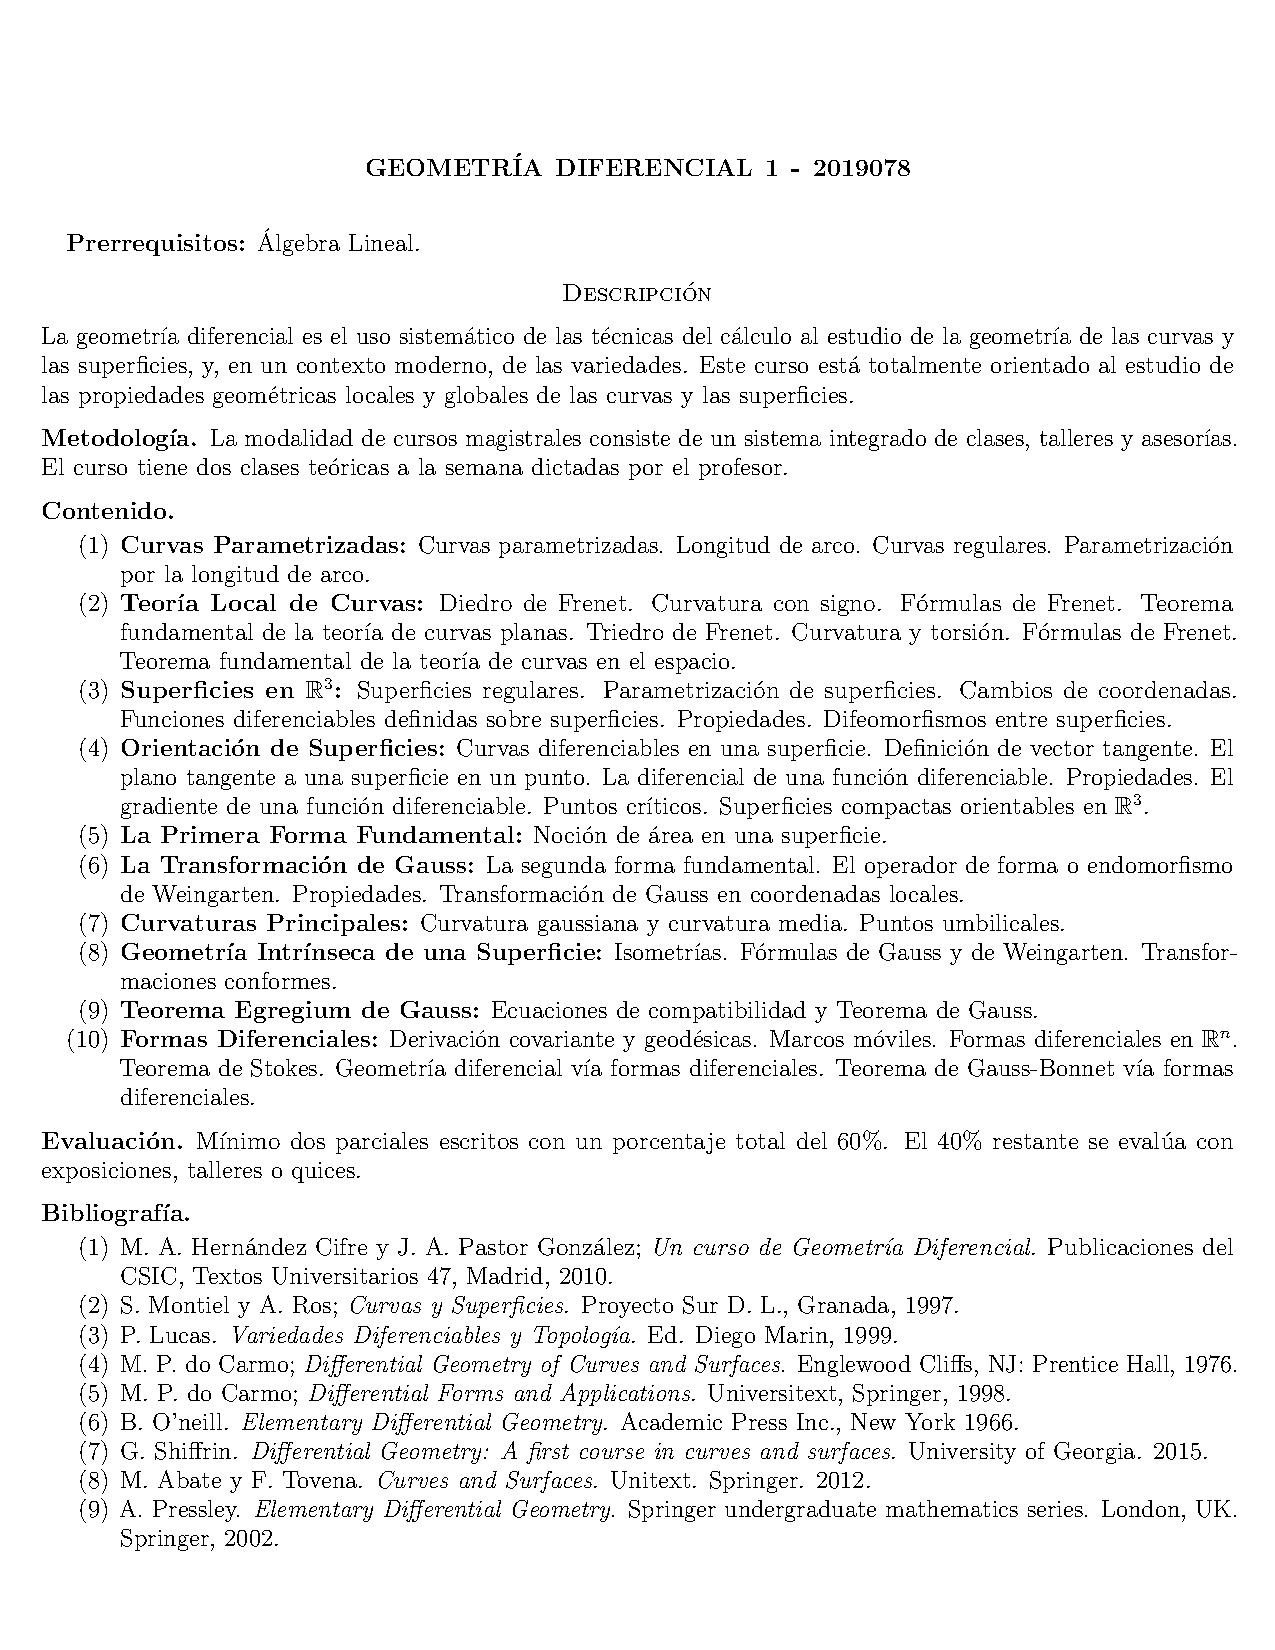
\includepdf[pages=-, fitpaper=true]{ProgramaGeoDif1.pdf}
\begin{itemize}
  \item Datos de la profesora.
  \item Calificación.
    \begin{itemize}
      \item $\%25$ Parcial I.
      \item $\%25$ Parcial II.
      \item $\%10$ Asistencia.
      \item $\%40$ Póster final. 
    \end{itemize}
\end{itemize}



% Índice
\tableofcontents

\chapter{Matrices.}
Una gran cantidad de los problemas que quizás el lector ha visto hasta el día de hoy tienen que ver con ecuaciones que relacionan variables entre sí. Una ecuación de este estilo es
\begin{align*}
  ax=b,
\end{align*}
que lo que busca es expresar la variable $b$ en términos de la variable $x$ y la constante $a$, se denomina \textbf{ecuación lineal}. El término lineal viene de como se puede representar gráficamente la ecuación anterior.\\
Note que problemas similares se pueden extender a más variables de la siguiente forma:
\begin{equation}\label{eq:1-lineal-n}
  a_1x_1+a_2x_2+\cdots+a_nx_n=b,
\end{equation}
que expresa a $b$ en términos de $x_1,x_2,\cdots$ y $x_n$ junto a las constantes $a_1,a_2,\cdots$ y $a_n$, de nuevo a este tipo de problemas se les denomina \textbf{ecuación lineal}.\\
Durante el desarrollo de estas notas nuestra intención será resolver problemas en los que se nos da $b$ y las constantes $a_1,a_2,\cdots$ y $a_n$ con el fin de encontrar $x_1,x_2,\cdots$ y $x_n$ denominados \textbf{incógnitas}, que resuelvan la ecuación $(\ref{eq:1-lineal-n})$.\\
Diremos que una colección de números $s_1,s_2,\cdots$ y $s_n$ son solución de $(\ref{eq:1-lineal-n})$ si al tomar $x_1=s_1,x_2=s_2,\cdots$ y $x_n=s_n$ se satisface que:
\begin{align*}
  a_1s_1+a_2s_2+\cdots+a_ns_n=b,
\end{align*}
Un breve ejemplo de esto podría ser tomar $x_1=2$ y $x_2=9$ en la ecuación
\begin{align*}
  2x_1+3x_2=31,
\end{align*}
ya que
\begin{align*}
  2(2)+3(9)&=4+27\\
  &=31.
\end{align*}
Ahora, con el fin de continuar con el desarrollo de manera más general diremos que un \textbf{sistema de $m$ ecuaciones lineales con $n$ incógnitas $x_1,x_2,\cdots$ y $x_n$} al que le llamaremos simplemente un \textbf{sistema lineal}, es un conjunto de $m$ ecuaciones lineales, cada una con $n$ incógnitas. Este mismo se podrá representar de la siguiente forma
\begin{equation}\label{eq:1-sistema-lineal}
  \begin{split}
    a_{11}x_1+a_{12}x_2+\cdots+a_{1n}x_n&=b_1\\
    a_{21}x_1+a_{22}x_2+\cdots+a_{2n}x_n&=b_2\\
    \vdots \hspace{1.3cm} \vdots \hspace{1.3cm} \vdots \hspace{1.3cm} \vdots &\phantom{=} \hspace{0.2cm}\vdots\\ 
    a_{m1}x_1+a_{m2}x_2+\cdots+a_{mn}x_n&=b_m
  \end{split}
\end{equation}
En dónde los subíndices $i$ y $j$ se usarán para mencionar la $i$-ésima ecuación y la $j$-ésima variable.\\
De nuevo diremos que una colección de $n$ números es solución de $(\ref{eq:1-sistema-lineal})$ si estás son a su vez solución de cada una de las $m$ ecuaciones.\\
Durante el desarrollo de las notas veremos algunos métodos que nos ayudarán a encontrar soluciones (en caso de haberlas) para problemas de este estilo, por ahora veamos un ejemplo.
\begin{example}
  El director de un fondo de inversión tiene \$100,000 para invertir. Las reglas del fondo establecen que la inversión debe hacerse tanto en certificados de depósito (CD), como a largo plazo. El objetivo del director es obtener un rendimiento de \$7,800 sobre las inversiones al cabo de un año. Los CD elegidos tienen un rendimiento de 5\% anual, mientras que el bono ofrece 9\% al año. El director determina cómo sigue la cantidad \( x \) que debe invertir en los CD, y la cantidad \( y \) que dedicará a comprar bonos:\\
  Como la inversión total es de \$100,000, debemos tener \( x + y = 100,000 \). Toda vez que el rendimiento deseado es de \$7,800, obtenemos la ecuación \( 0.05x + 0.09y = 7,800 \). Por lo tanto, tenemos el sistema lineal
  \begin{equation}\label{eq:1-3}
    \begin{aligned}
      x + y &= 100,000 \\
      0.05x + 0.09y &= 7,800.
    \end{aligned}
  \end{equation}
  Para eliminar \( x \), sumamos \( (-0.05) \) veces la primera ecuación a la segunda, para obtener
  \begin{align*}
    x + y &= 100,000 \\
    0.04y &= 2,800,
  \end{align*}
  en donde la segunda ecuación no tiene término \( x \); en otras palabras, hemos eliminado la incógnita \( x \). Después despejamos \( y \) en la segunda ecuación, para obtener
  \begin{align*}
    y=70,000,
  \end{align*}
  y sustituyendo \( y \) en la primera ecuación de $(\ref{eq:1-3})$, obtenemos
  \begin{align*}
    x=30,000.
  \end{align*}
  Para comprobar que \( x = 30,000, y = 70,000 \) es una solución de (3), verificamos que estos valores de \( x \) y \( y \) satisfagan \textit{cada una} de las ecuaciones del sistema lineal dado. En consecuencia, el director del fondo debe invertir \$30,000 en los CD y \$70,000 en bonos a largo plazo.
\end{example}


\chapter{Determinantes.}
\chapter{Vectores en $\mathbb{R}^{n}$.}
\chapter{Espacios vectoriales reales.}
\chapter{Valores propios, vectores propios y diagonalización.}
\section{Valores y vectores propios.}
A partir de este momento solo hablaremos de matrices cuadradas $n\times x$. Recordemos que si tomamos una matriz $A$ podemos definir $L(\x)=A\x$ con $\x\in\mathbb{R}^{n}$ como una transformación lineal. Una buena pregunta será ver si existen vectores $\x$ tales que $A\x$ y $\x$ son paralelos, esto nace de varias aplicaciones en distintas áreas del saber.
\begin{definition}
  Sea $A$ una matriz $n\times n$. El número real $\lambda$ es un \textbf{valor propio} (o \textbf{valor característico o autovalor}) de $A$ si existe un vector $\x$ distinto de $0$ en $\mathbb{R}^{n}$ tal que
  \begin{equation}\label{eq:5-valor-propio}
    A\x=\lambda\x.
  \end{equation}
  A su vez todo vector que cumpla $(\ref{eq:5-valor-propio})$ es un \textbf{vector propio} asociado al valor propio $\lambda$, su nombre puede variar de la misma forma que los valores propios. 
\end{definition}
\begin{note}
  En otros contextos $\lambda$ y $\x$ se pueden tomar tanto reales como complejos. 
\end{note}
\begin{note}
  Note que un mismo valor propio de $A$ puede tener asociados muchos vectores propios, pues si suponemos que $\x$ es un vector propio asociado a $\lambda$, entonces 
  \begin{align*}
    A(r\x)&=rA\x,\\
    &=r\lambda\x,\\
    &=\lambda(r\x).
  \end{align*}
\end{note}
\begin{example}
  Sea
  \begin{align*}
    A = \begin{pmatrix}
      0 & 0 \\
      0 & 1
    \end{pmatrix}
    .
  \end{align*}
  Note que
  \begin{align*}
    A \begin{pmatrix}
      1 \\
      0
    \end{pmatrix}
    &=\begin{pmatrix}
      0 & 0 \\
      0 & 1
    \end{pmatrix}
    \begin{pmatrix}
      1 \\
      0
    \end{pmatrix},\\
    &=\begin{pmatrix}
      0 \\
      0
    \end{pmatrix}
    ,\\
    &=0 \begin{pmatrix}
      1\\
      0
    \end{pmatrix}
    .
  \end{align*}
  De lo que podemos ver que $\lambda=0$ es un valor propio de $A$ (verifique esto con la definición). 
\end{example}
A groso modo, note que cuando queremos hallar los valores propios de una matriz $A$ en general nos cruzamos con una ecuación como la siguiente.
\begin{align*}
  \begin{pmatrix}
    a & b \\
    c & d
  \end{pmatrix}
  \begin{pmatrix}
    x_1 \\
    x_2
  \end{pmatrix}
  =\lambda \begin{pmatrix}
    x_1 \\
    x_2
  \end{pmatrix}
  .
\end{align*}
Lo que en general se puede ver como
\begin{align*}
  \begin{cases}
    ax_1+bx_2=\lambda x_1, \\
    cx_1+dx_2=\lambda x_2.
  \end{cases}
\end{align*}
lo cual se puede llevar a
\begin{align*}
  \begin{cases}
    (a-\lambda)x_1+bx_2=0, \\
    cx_1+(d-\lambda)x_2=0.
  \end{cases}
\end{align*}
Luego como esto es un sistema homogéneo de 2 ecuaciónes con 2 incógnitas podemos afirmar que este tiene solución no trivial si y sólo si el determinante respectivo es distinto de $0$, es decir
\begin{align*}
  \begin{bmatrix}
    a-\lambda & b \\
    c & d-\lambda
  \end{bmatrix}\neq 0.
\end{align*}
Lo que de puede escribir como $det(A-\lambda I)$, vamos a extender esto en general para cualquier matriz $A$ $n\times n$.
\begin{definition}
  Sea $A$ una matriz $n\times n$, definimos $f(\lambda)=det(A-\lambda I)$ como el \textbf{polinomio característico} de $A$.\\
  Así mismo definiremos $f(\lambda)=0$ como la \textbf{ecuación característica} de $A$. 
\end{definition}
\begin{theorem}
  Una matriz $n\times n$ es singular si y sólo si $0$ es un valor propio. 
\end{theorem}


% Bibliografía
\bibliographystyle{plainnat}
\bibliography{references}  

\end{document}

